\documentclass[a4paper,11pt]{article}
\usepackage[margin=1in]{geometry}
\usepackage{graphicx}
\usepackage{parskip}
\usepackage{hyperref}
\usepackage{enumitem}
\usepackage{newtxtext} % Use Times New Roman font
\usepackage[pro]{fontawesome5}
\usepackage{xcolor}

% Define ORCID green
\definecolor{orcid}{RGB}{166, 206, 57}

\setlength{\parindent}{0pt} % Remove paragraph indent
% not hyperlink the email and phone number
\hypersetup{
    colorlinks = true,
    urlcolor = blue
}
\newcommand{\pKa}{p\textit{K}\textsubscript{a}}
\begin{document}

\begin{minipage}[c]{0.75\textwidth} % Right side for the details
    {\Huge \textbf{\textit{CURRICULUM VITAE}}}\vspace{1cm}\\
    {\Huge \textbf{Shijie Xu}}\vspace{1cm}\\
    Faculty of Environmental Earth Science, Hokkaido University\\
    Kita-10 Nishi-5, Kita-ku, Sapporo, Hokkaido, 060-0810, Japan\\

    \faEnvelope~\href{mailto:shijie.xu@ees.hokudai.ac.jp}{shijie.xu@ees.hokudai.ac.jp}~~~\color{orcid}{\faOrcid}~\href{https://orcid.org/0000-0001-6974-353X}{0000-0001-6974-353X}
\end{minipage}
\hfill
% Header with Photo
\begin{minipage}[c]{0.2\textwidth} % Left side for the photo
    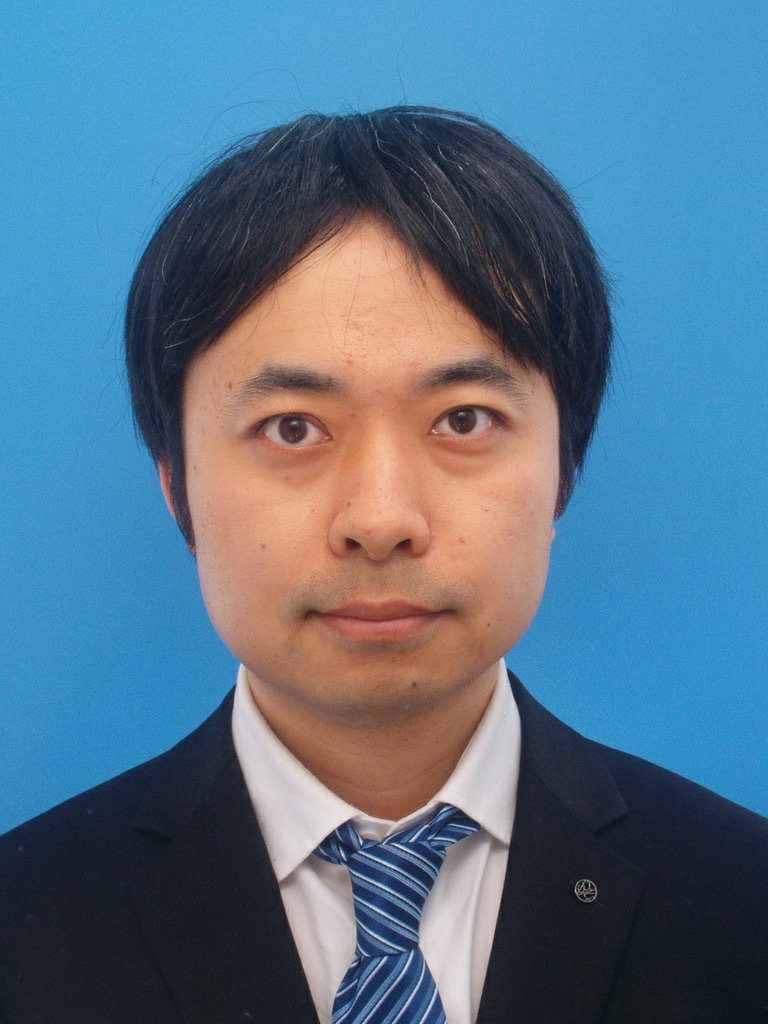
\includegraphics[width=\linewidth]{profile.JPG} % Replace "photo.jpg" with your photo file
\end{minipage}

\vspace{0.5cm}

\section*{Date of Birth}
March 9th, 1995
% Education
\section*{Education}
Ph.D. in Environmental Science, Hokkaido University \hfill March 2025\\
\textit{Dissertation Title: ``Accurate and Fast Predictions of Protein\\
Structures and Properties via Protein Language Models''}\\
M.S. in Computer Science, University of Science and Technology of China \hfill June 2020\\
B.S. in Mathematics, University of Science and Technology of China \hfill June 2017
\section*{Research Experience}
Postdoctoral Researcher, Hokkaido University\hfill April 2025 - Present\\

\section*{Research Interests}
Bioinformatics, Deep Learning, Computational Chemistry, Computer Science, Mathematics
\section*{Skills}
\textbf{Programming:} Python / C++ / \LaTeX / FORTRAN / Rust / Mathematica / MATLAB / Coq / Haskell\\
\textbf{Web development:} HTML / JavaScript / FastAPI / Flask / Django / Go\\
\textbf{Software:} AutoDock Vina / PyMOL / GIMP / Git / Docker / VSCode\\
\textbf{Hardware:} GPU workstation building / Linux server maintenance / Raspberry Pi\\
\textbf{Languages:} English (fluent), Chinese (standard and lower Yangtze), Japanese (basic)
\section*{Publications}
\begin{enumerate}
    \item \underbar{Shijie Xu} and Akira Onoda*. ``PsiPartition: Improved Site Partitioning for Genomic Data by Parameterized Sorting Indices and Bayesian Optimization.'' \textit{Journal of Molecular Evolution} 92: 874-890, \textbf{2024}, \emph{DOI:} \url{https://doi.org/10.1007/s00239-024-10215-7}
    \item \underbar{Shijie Xu} and Akira Onoda*. ``Accurate and Fast Prediction of Intrinsically Disordered Protein by Multiple Protein Language Models and Ensemble Learning.'' \textit{Journal of Chemical Information and Modeling} 64(7): 2901-2911, \textbf{2023}, \emph{DOI:} \url{https://doi.org/10.1021/acs.jcim.3c01202} 
    \item \underbar{Shijie Xu} and Akira Onoda*. ``Accurate and Rapid Prediction of Protein \pKa{}: Protein Language Models Reveal the Sequence-\pKa{} Relationship.'' \textit{Journal of Chemical Theory and Computation}
\end{enumerate}
\section*{Presentations}
\begin{itemize}
    \item \underbar{Shijie Xu} and Akira Onoda, ``Accurate and Fast Prediction of Protein \pKa{} by Protein Language Model,'' 8th ICReDD International Symposium, 22nd Oct - 24th Oct 2024, Sapporo, Japan. [Poster]
    \item \underbar{Shijie Xu} and Akira Onoda, ``Accurate Prediction of Intrinsically Disordered Protein by Protein Language Models,'' the 24th Annual Meeting of the Protein Science Society of Japan, 11th Jul - 13th Jul 2024, Sapporo, Japan. [Poster]
    \item \underbar{Shijie Xu} and Akira Onoda, ``Accurate Prediction of Protein \pKa{} by Geometric Deep Learning,'' the 104th CSJ annual meeting, 18th Mar - 21st Mar 2024, Funabash, Japan. [Oral]
    \item \underbar{Shijie Xu} and Akira Onoda, ``Accurate Prediction of Intrinsically Disordered Protein by Protein Language Models,'' the 17th Biorelevant Chemistry Symposium, 8th Sep - 10th Sep 2023, Chiba, Japan. [Poster]
    \item \underbar{Shijie Xu} and Akira Onoda, ``Fast and Accurate Prediction of Intrinsically Disordered Protein by Protein Language Model,'' the 103rd CSJ annual meeting, 22nd Mar - 25th Mar 2023, Chiba, Japan. [Oral] 
\end{itemize}
\section*{Awards, Fellowships, and Grants}
\begin{itemize}
    \item Program for Supporting Challenging and Interdisciplinary Research Field, 2022, 2023, 2024
    \item Hokkaido University DX Doctoral Fellowship, 2022-2025
    \item Outstanding Student Scholarship, University of Science and Technology of China, 2016
    \item S.-T. Yau College Student Mathematics Contests, Beijing, China, 2016
    \item Outstanding Freshman Scholarship, University of Science and Technology of China, 2014
    \item First Prize Winner in National High School Mathematics League, Hefei, Anhui, China, 2012
\end{itemize}

\end{document}
